%!TEX root = ../CombinatoricsNotes.tex

\section{Set systems as an introduction to extremal combinatorial results}\marginnote{The following is a brief introduction to some of the results we will see in the course. 

Note that the superscripted symbols $^\dagger$, $^\ddagger,$ and $^*$ are reserved to point towards notes in this margin. 

In this introduction, full references will be included in the margin; afterwards, they will appear at the end of each section.}
 A \emph{set system} is any $\F\subset \P(X)$.
Let $X$ be a finite set, and $\P(X)$ the collection of all subsets of $X$.  Then $|\P(X)|  = 2^{|X|}$. We'll denote $X^{(r)}$ as the collection of all $r$-element subsets of $X$.
\begin{example}
If $X = \{1,2,3\}$, then $\P(X)=$ 
\begin{center}
 \begin{tikzcd}
X^{(3)}  & &\{1,2,3\} \\
X^{(2)} &\{1,2\} & \{1,3\} & \{2,3\} \\
X^{(1)} & \{1\} & \{2\}&\{3\} \\
X^{(0)} & & \emptyset
\end{tikzcd}
\end{center}
\end{example}


\begin{definition}
$\F$ is an \defn{intersecting set system} if $A\cap B\neq\emptyset$ for all $A,B\in \F$.
\end{definition}

\subsection*{Largest intersecting set system}
Given $X$ with $|X| = n$, what is the maximum $|\F|$ with $\F\subset \P(X)$ intersecting? Let's start with $n=3$ (returning to our example). We can select at least 4: every set that contains 1\marginnote{In this case, we could also choose $X^{(2)}\cup X^{(3)}$, but that only works for $n$ odd.}. This method gives us $2^{n-1}= |\P(X \setminus\{1\})|$\sidenote{since the number of subsets without 1 is in bijection with the number of subsets with 1. For a subset without 1, we add in 1, and get a new valid subset with 1. On the other hand, for a subset with 1, we take out 1 and get a valid subset without 1. These are clearly injective.}. Why can't we do better? We can subdivide $\P(X)$ into pairs $\{Y, X\setminus Y\}$. But $Y\cap (X\setminus Y) = \emptyset$, so any intersecting $\F$ contains at most one element of each pair. Thus, we can't do better than $2^{n-1}$.

\subsection*{Largest intersecting set system with fixed number of elements}
How large can $\F$ intersecting be if $\F\subset X^{(r)}$ for some $r$? Our answer will depend on $r$ and $|X| = n$. Since $|X^{(r)}| = {n \choose r}$, that is an upper bound. When can we achieve it, i.e. when is $X^{(r)}$ intersecting? When $r > n/2$. In this case, every subset has more than half of the elements of $X$, so no two subsets can be disjoint.

If $r = n/2$, then because of  complement pairing, the maximum is ${n \choose r}/2$. By choosing $\F$ as all of the sets that contain a particular element, we get ${n -1\choose r-1}$. So for $r=n/2$, we have
\[
 {n-1\choose r-1} \leq \max |\F| \leq \frac{1}{2}{n\choose r}.
\]
But for $r=n/2$, these two bounds are equal\sidenote{Why? the LHS is the number of sets containing 1. But half of the sets contain 1 and half don't, by the complement argument.}.
For $r< n/2$, the answer is ${n -1 \choose r-1}$; this is a lower bound by selecting all sets containing a given element.  That this is an upper bound is the content of the following non-trivial theorem.
\begin{theorem*}[\erdos-Ko-Rado] \marginnote{\fullcite{erdos-ko-rado-1961}}
Let $r\leq n/2$. Let $\F\subset X^{(r)}$ with $|X| = n$ be intersecting. Then $|F| \leq { n-1\choose r-1}$.
\end{theorem*}

Next, let's consider other types of set systems.
\subsection*{Littlewood-Offord problem}
We'll say $\F$ is a \defn{Sperner system} if $A\subset B$ for $A,B\in \F$, then  $A=B$.
Given $X$, $|X|=n$, what is $\max |\F|$ such that $\F\subset \P(X)$ is Sperner? Well, any $X^{(r)}$ is Sperner\sidenote{If you take any element out, you reduce the number of elements, so aren't in $X^{(r)}$ anymore.}. So we can achieve ${n \choose \floor{n/2} }$. It turns out that one cannot do better. For $n=3$, we may make a graph by connecting subsets by edges. Then we need the largest independent set of this graph; it's easy to show in this case that this is ${n \choose \floor{n/2} }$. This is in fact the general result.
\begin{problem}[Littlewood-Offord 1938] \marginnote{\fullcite{LO1943}}
Suppose we have non-zero numbers $a_1,a_2,\ldots,a_n \in \C$. For $I\subset \{1,2,\dotsc,n\}$, consider $\sum_{i\in I} a_i$. There are then $2^n$ possible such sums. What is the maximal number of them that can be equal to be zero? 
\end{problem}
Clearly we can shift to any number $z$ instead of zero without changing the answer.  \erdos\ solved this in 1945 for real numbers. Let's consider the case of positive numbers. 
First, if $a_1=\dotsm = a_n=1$, then the maximum number of equal sums is ${n \choose \floor{n/2} }$. 
Now for general positive numbers, consider $\F_z = \{ I: \sum_{i\in I} a_i = z\}$. Then $\F_z$ is a Sperner system, so by the previously quoted result its maximum size is ${n \choose \floor{n/2} }$.
The Littlewood-Offord problem was treated in general in 1966 by Kleitman\footfullcite{KLEITMAN1970}.

\subsection*{\erdos-Szemer\'edi conjcture}
% \begin{conjecture}[]
Let $A\subset \Z_+$, $|A| = n$. Let $A+A = \{ a+b: a,b\in A\}$. We wish to compare $|A+A|$ to $|A|$.
Now, $\max |A+A| = {n \choose 2} + n = {n+1 \choose 2}$ by choosing our elements so no two sums are the same unless they have to be\sidenote{Intuitively then, we've achieved the maximum by a set with very little structure.}.

What is $\min|A+A|$?
We'll choose a set with a lot of structure: $A= \{1,\dotsc,n\}$. Then $A+A = \{2,3,\dotsc,2n\}$, and $|A+A| = 2n-1$. We'll prove that this is actually the minimum.
% \end{conjecture}
\begin{proof}  
Let $a_1  < a_2  <\dotsm < a_n$\marginnote{The elements are distinct because $A$ is a set.}. Then
\[
\underbrace{a_1 + a_1 < a_1 + a_2 < \dotsm < a_1 + a_n}_{n} < \underbrace{a_2 + a_n < a_3 + a_n < \dotsm < a_n + a_n}_{n-1}
\]
so we found $2n-1$ different terms already.
\end{proof}

What about $|A\cdot A|$? Then $\max |A\cdot A| = {n\choose 2} +n$, and $\min |A\cdot A| = 2n-1$. The second is by $A = \{1,2,2^2,\dotsm, 2^{n-1}\}$. Generally we can transform additive problems into multiplicative by exponentiation, and back by the logarithm.
Now, what's $\min ( |A+A| + |A\cdot A|)$? 
\begin{conjecture*}[\erdos-Szemer\'edi] \marginnote{\fullcite{Erdos-Szemeredi-1983}}
\marginnote{This qualitatively means the additive and multiplicative structures do not get along; you reduce $|A+A|$ only at the cost of increasing $|A\cdot A|$.}
\[
|A+A| + |A\cdot A| = \Omega_\epsilon (|A|^{2-\epsilon})
\]
That is, for all $\epsilon>0$, there exists $c>0$ such that for all $A\subset \Z_+ \setminus \{0\}$,
\[
|A + A| + |A\cdot A| \geq c_\epsilon |A|^{2- \epsilon}.
\]
\end{conjecture*}
Elekes showed that $|A +A| + |A\cdot A| \geq c |A|^{5/4}$ (\cite{elekes1997number}) and Solymosi improved this to bound to  $|A|^{4/3 - \epsilon}$~(\cite{Solymosi2009}).
In fact, this is related to the following geometric problem (see \cref{fig:IPLexample} for an example).
\begin{theorem*}[Szemer\'edi-Trotter theorem] \marginnote{\fullcite{Szemeredi-Trotter1983}}
\begin{marginfigure}[2cm]
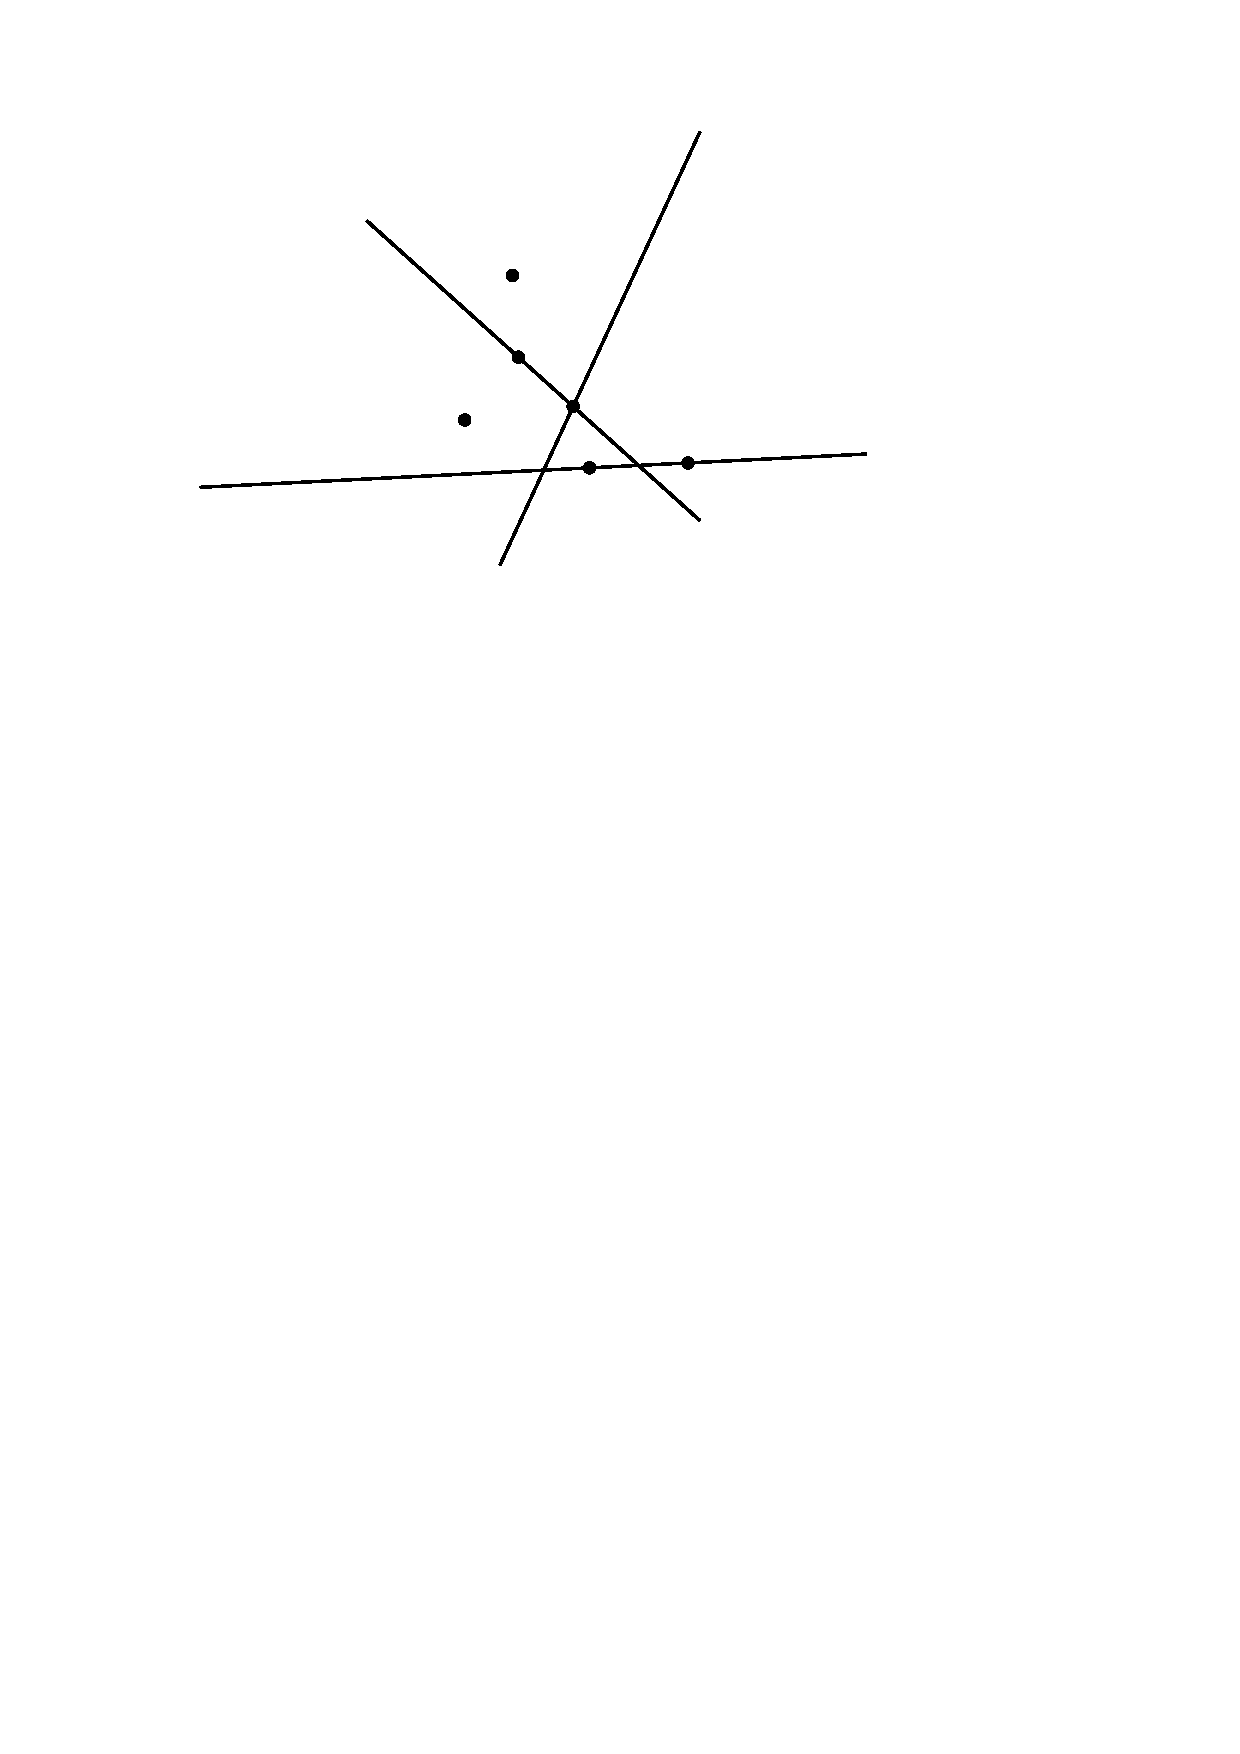
\includegraphics{L1f1.pdf}
\caption{An example of a collection $L$ of lines and $P$ of points. We are interested in the number of \defn{incidences} $I(P,L)$ between points in $P$ and lines in $L$. Here, $I(P,L) = 5$.} \label{fig:IPLexample}
\end{marginfigure}
Suppose we have a collection $L$ of lines in the plane, and $P$ a collection of points in the plane. The set of incidences is $\{(p,\ell): p\in P, \ell\in L, p\in \ell\}$.   Let $I(P,L)$ denote the number of incidences for $P$ and $L$\sidenote{Clearly, $I(P,L) \leq |P| \cdot |L|$, as a subset of $P\times L$.}. Then
\[ 
I(P,L) \leq O ( |P|^{2/3} |L|^{2/3} + |P| + |L| ).
\]
\end{theorem*}
Elekes used this theorem to make progress on the \erdos-Szemer\'edi conjecture by mapping the set $A$ to a collection of points and lines. He showed that if both $|A\cdot A|$ and $|A+A|$ are small, then you find too many incidences.
The Szemer\'edi-Trotter theorem uses the following result:
\begin{lemma*}[Crossing lemma]
Let $G$ be a graph drawn in the plane with crossings. Suppose that $G$ has $m$ edges and $n$ verticies\marginnote{If $m > 3n-6$, then there is at least one crossing, by the result stated at the beginning of the lecture, which comes from Euler's formula. In fact, this is how one proves the crossing lemma.}. If $m\geq 4n$, then there are at least $\frac{m^3}{64 n^2}$ crossings.
\end{lemma*}
From $P$ and $L$, one makes a graph and applies the Crossing Lemma to prove Szemer\'edi-Trotter.
